% Uncomment this to make slides with overlays:
\documentclass[slides]{beamer}

% Uncomment these (but comment the above \documentclass line) to make handouts:
%\documentclass[handout]{beamer}

% Uncomment these to have more than one slide per page
%\usepackage{pgfpages}
%\pgfpagesuselayout{2 on 1}[border shrink=5mm]
%\pgfpageslogicalpageoptions{1}{border code=\pgfusepath{stroke}}
%\pgfpageslogicalpageoptions{2}{border code=\pgfusepath{stroke}}

\usepackage[]{graphicx, color, hyperref}

\mode<presentation>
{
	%\usetheme[secheader]{Boadilla}
	%\usecolortheme[rgb={.835, .102,.169}]{structure}  
	\usetheme[width= 0cm]{Goettingen}
	%\setbeamercovered{transparent}
}
\setbeamertemplate{navigation symbols}{}
\setbeamertemplate{footline}[frame number]

\definecolor{blue2}{rgb}{0.278,0.278,0.729} 
\newcommand{\blue}[1]{\textcolor{blue2}{#1}}
\newcommand{\white}[1]{\textcolor{white}{#1}}
\newcommand{\red}[1]{\textcolor{red}{#1}}
\newcommand{\xbar}{\overline{x}}
\newcommand{\ybar}{\overline{y}}
\newcommand{\phat}{\widehat{p}}
\newcommand{\prob}{\mbox{Pr}}
\newcommand{\E}{\mathbb{E}}
\newcommand{\Var}{\mbox{Var}}
\newcommand{\cp}{\oplus}
\newcommand{\cm}{\circleddash}


\title{Lecture 17: Paired Data and Difference of Two Means}
\author{Chapter 5.1-5.2}
\date{}


\begin{document}
%------------------------------------------------------------------------------
\begin{frame}
\titlepage
\end{frame}
%------------------------------------------------------------------------------



%------------------------------------------------------------------------------
\begin{frame}[fragile]
\frametitle{Goals for Today}

\begin{itemize}
\item Define statistical power
\item Difference of Means
\item Note on Practical vs Statistical Significance
\end{itemize}

\end{frame}
%------------------------------------------------------------------------------






%-------------------------------------------------------------------------------
\begin{frame}
\frametitle{The 8 Types of Questions}

Here are the 8 broad types of questions we can answer with statistical methods (confidence intervals and hypothesis tests) in this class: 

\vspace{0.25cm}

\begin{enumerate}
\pause\item What is the mean value $\mu$?
\pause\item Are the means of two groups $\mu_1$ and $\mu_2$ equal or not?
\pause\item What is the mean paired difference $\mu_{diff}$?
\pause\item What is the proportion $p$ of ``successes''?
\pause\item Are the proportions of ``successes'' of two groups $p_1$ and $p_2$ equal or not?
\pause\item Are the means $\mu_1, \ldots, \mu_k$ of $k$ groups \blue{all} equal or not?
\pause\item Are we observing counts that we were expected?
\pause\item Are two categorical variables independent?
\end{enumerate}

\end{frame}
%-------------------------------------------------------------------------------







%total <- hist(run10Samp$time)
%F <- hist(run10Samp$time[run10Samp$gender=="F"])
%M <- hist(run10Samp$time[run10Samp$gender=="M"])
%
%mean.m <- mean(run10Samp$time[run10Samp$gender=="M"])
%mean.f <- mean(run10Samp$time[run10Samp$gender=="F"])
%
%pdf("./7.3 Paired Data + Diff of Two Mean/race.pdf", width=6, height=6)
%hist(run10Samp$time[run10Samp$gender=="M"], breaks=total$breaks, col='cyan',
%     border='cyan', xlab="Race Time (in minutes)", main="Cherry Blossom Run Times", 
%     ylim=c(0,max(F$counts, M$counts)))
%hist(run10Samp$time[run10Samp$gender=="F"],add=T)
%legend("topright", 
%       legend=c("men", "women"), 
%       fill=c("cyan", "white"),
%       bty='n')
%dev.off()
%------------------------------------------------------------------------------
\begin{frame}[fragile]
\frametitle{Are the means of two groups $\mu_1$ and $\mu_2$ equal or not?}

Example from Chapter 5.2:  Did men (n=45) run faster than women (n=55)?
\begin{center}
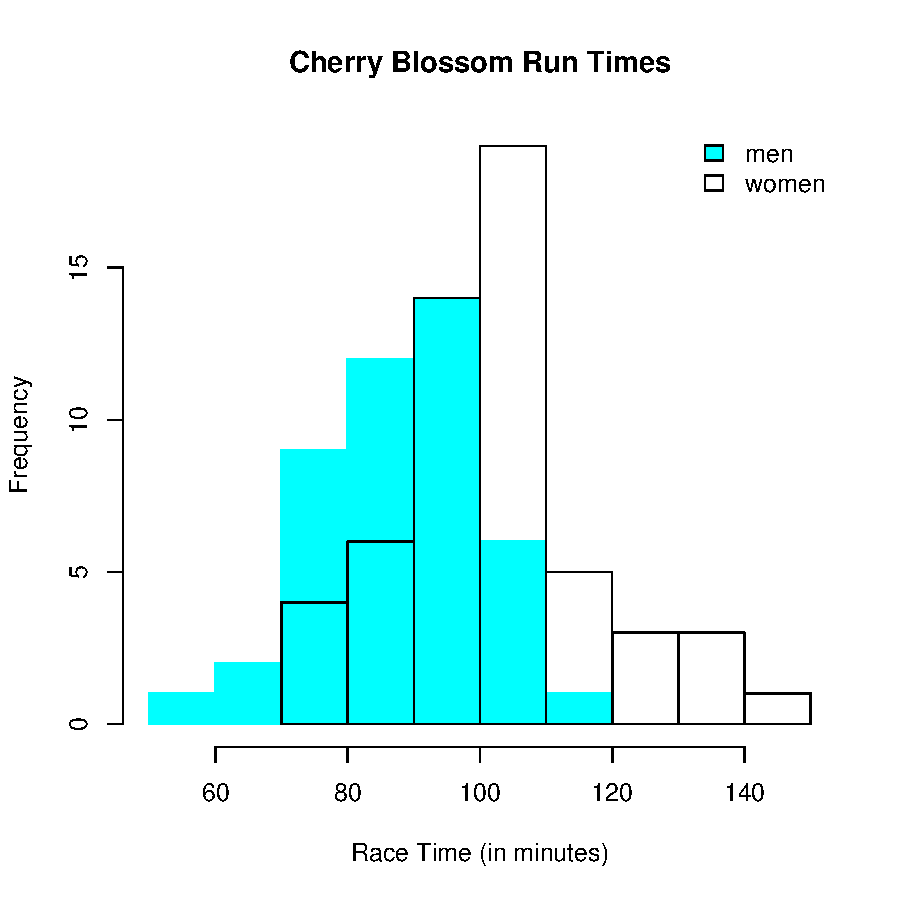
\includegraphics[width=0.6\textwidth]{figure/race.pdf}
\end{center}

\end{frame}
%------------------------------------------------------------------------------


%------------------------------------------------------------------------------
\begin{frame}[fragile]
\frametitle{Difference in Means}
We are interested in the difference of two population means $\mu_w - \mu_m$ where
\pause\begin{itemize}
\item $\mu_w$ is the mean time for women
\item $\mu_m$ is the mean time for men
\end{itemize}

\pause\vspace{0.5cm}
The data:
\begin{center}
  \begin{tabular}{c|rr}
     & men & women \\ 
\hline
    $\overline{x}$ & 87.65 & 102.13 \\ 
    $s$ & 12.5 & 15.2 \\ 
    $n$ & 45 & 55 \\ 
\end{tabular}
\end{center}

\end{frame}
%------------------------------------------------------------------------------


%------------------------------------------------------------------------------
\begin{frame}[fragile]
\frametitle{Difference of Means}
We now recreate all the elements of Chapter 4 using this new \blue{population parameter}  $\mu_w - \mu_m$:

\vspace{0.25cm}

\begin{enumerate}
\pause\item Determine a point estimate of $\mu_w - \mu_m$.
\pause\item Show the normality of the sampling distribution:  mean and SE
\pause\item Build a confidence interval
\pause\item Conduct hypothesis tests
\end{enumerate}

\vspace{0.25cm}

\pause First, the \blue{point estimate} for $\mu_w - \mu_m$ is the \blue{sample difference of means}
\[\xbar_w - \xbar_m = 102.13-87.65=14.48\]



\end{frame}
%------------------------------------------------------------------------------


%------------------------------------------------------------------------------
\begin{frame}[fragile]
\frametitle{Normality of Sampling Distribution}
If the sample means $\xbar_1$ and $\xbar_2$ 
\begin{itemize}
\pause\item each meet the criteria for having nearly normal sampling distributions
\pause\item also \blue{the observations from the two samples are independent}
\end{itemize}
\pause then the difference in sample means $\xbar_1 - \xbar_2$ will also have a nearly normal sampling distribution...

\end{frame}
%------------------------------------------------------------------------------


%------------------------------------------------------------------------------
\begin{frame}[fragile]
\frametitle{Normality of Sampling Distribution}
with 
\begin{itemize}
\pause\item mean $\mu_1-\mu_2$
\pause\item estimated standard error
\[
SE_{\xbar_1 - \xbar_2} = \sqrt{\frac{s_1^2}{n_1} + \frac{s_2^2}{n_2}}
\]
\end{itemize}
\pause Note the different $s^2$'s and sample sizes.  
\end{frame}
%------------------------------------------------------------------------------



%------------------------------------------------------------------------------
\begin{frame}[fragile]
\frametitle{Normality of Sampling Distribution}

We verify the conditions:
\begin{itemize}
\pause\item Because each sample consists of less than 10\% of their respective populations (men: 45 of 7192 and women: 55 of 9732).
\pause\item The observations for both groups don't look too skewed.
\pause\item Each sample has at least 30 observations (rule of thumb).
\pause\item The samples are independent (not paired or linked in any way).
\end{itemize}


\pause\vspace{0.25cm}
the sampling distribution is Normal with mean=$\mu_w - \mu_m$ and
\[
SE_{\xbar_w - \xbar_m} = \sqrt{\frac{15.2^2}{55} + \frac{12.5^2}{45}} = 2.77
\]

\end{frame}
%------------------------------------------------------------------------------




%------------------------------------------------------------------------------
\begin{frame}[fragile]
\frametitle{Confidence Interval}

A 95\% confidence interval for $\mu_1 - \mu_2$ is
\begin{eqnarray*}
(\mbox{point estimate for } \mu_1 - \mu_2) \pm 1.96 \times SE\\
\pause(\xbar_1 - \xbar_2) \pm 1.96 \times SE_{\xbar_1 - \xbar_2}
\end{eqnarray*}

\pause So for the Cherry Blossom Run data, a 95\% CI for $\mu_w - \mu_m$ is:
\begin{eqnarray*}
14.48 \pm 1.96 \times 2.77 =  [9.05, 19.91]
\end{eqnarray*}

\end{frame}
%------------------------------------------------------------------------------








%------------------------------------------------------------------------------
\begin{frame}[fragile]
\frametitle{Chapter 5.1: Paired Data}
Two sets of observations are \blue{paired} if each observation in one set has a special correspondence or connection with exactly one observation in the other data set.

\vspace{0.25cm} 

\pause Examples:

\begin{itemize}
\item Cholesterol levels before and after some intervention
\pause \item Disease rates amongst pairs of twins
\pause \item In the text:  price of the same textbook at the UCLA bookstore vs Amazon
\end{itemize}

\end{frame}
%------------------------------------------------------------------------------



%pdf("./7.3 Paired Data + Diff of Two Mean/diff.pdf", width=7, height=5)
%plot(textbooks$uclaNew, pch=19, log='y', xlab="Textbook #", ylab="Price",
%     main="UCLA & Amazon Price for Each Textbook")
%points(textbooks$amazNew, pch=19, col="red")
%legend("topleft", legend=c("UCLA","Amazon"), pch=c(19,19), col=c(1,2))
%dev.off()
%
%pdf("./7.3 Paired Data + Diff of Two Mean/diff2.pdf", width=7, height=5)
%plot(textbooks$uclaNew - textbooks$amazNew, pch=19, 
%     xlab="Textbook #", ylab="Difference in Price",
%     main="UCLA Price - Amazon Price")
%abline(h=0)
%dev.off()
%
%pdf("./7.3 Paired Data + Diff of Two Mean/diff2.pdf", width=7, height=5)
%boxplot(textbooks$uclaNew - textbooks$amazNew, horizontal=TRUE, xlab="UCLA Price - Amazon Price")
%dev.off
%------------------------------------------------------------------------------
\begin{frame}[fragile]
\frametitle{Paired Differences}
The methodology for paired data remains the same, except our \blue{observations} are the difference in pairs.  Example, for the UCLA Bookstore vs Amazon book price example in the text
\begin{center}
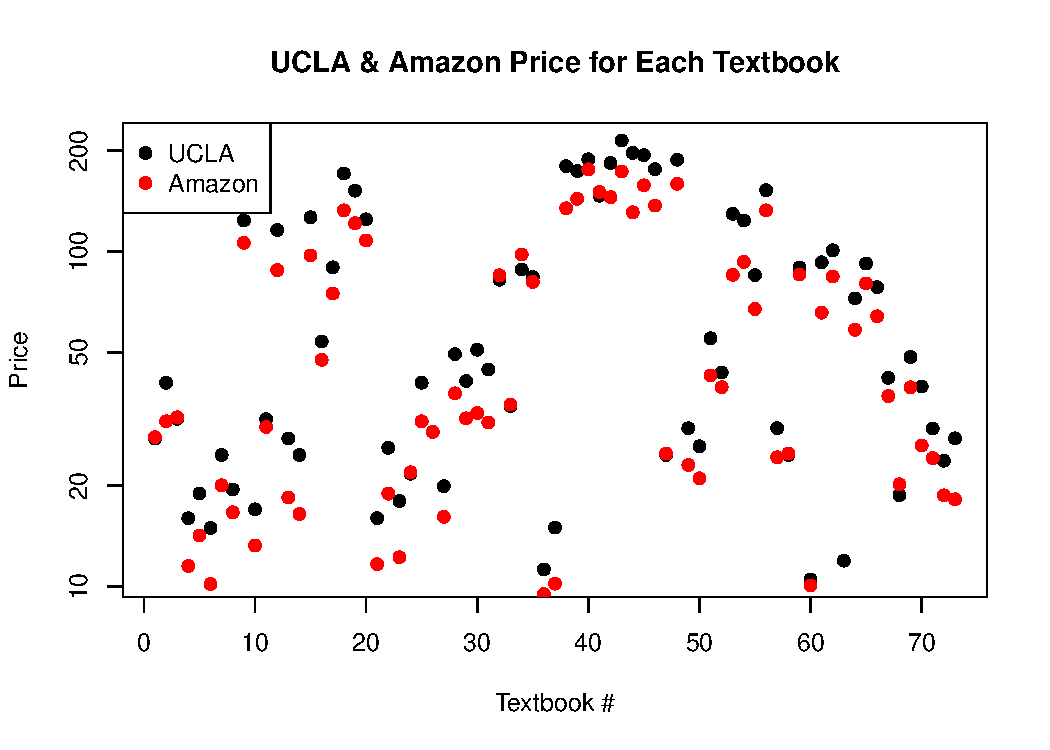
\includegraphics[width=0.8\textwidth]{diff.pdf}
\end{center}


\end{frame}
%------------------------------------------------------------------------------



%------------------------------------------------------------------------------
\begin{frame}[fragile]
\frametitle{Paired Differences}
The methodology for paired data remains the same, except our \blue{observations} are the difference in pairs.  Example, for the UCLA Bookstore vs Amazon book price example in the text
\begin{center}
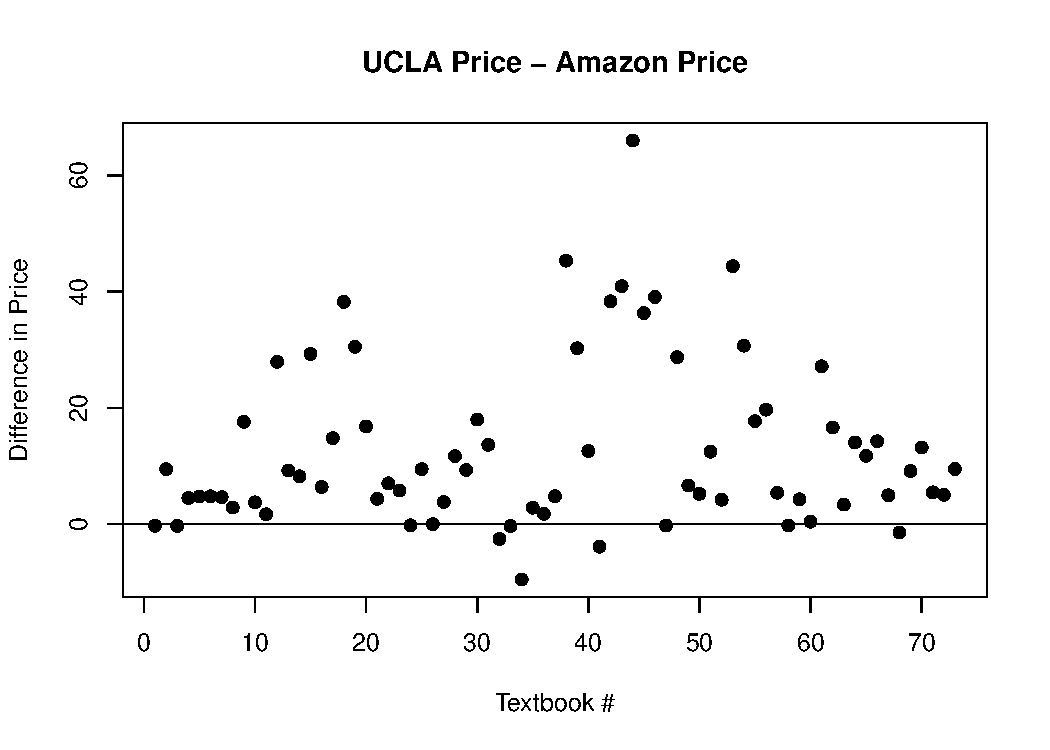
\includegraphics[width=0.8\textwidth]{diff2.pdf}
\end{center}


\end{frame}
%------------------------------------------------------------------------------



%------------------------------------------------------------------------------
\begin{frame}[fragile]
\frametitle{Paired Differences}
We have
\begin{itemize}
\pause \item population parameter is $\mu_{diff}$
\pause \item point estimate $\xbar_{diff}$ of $\mu_{diff}$
\pause \item Conditions: not on the original observations, but rather the \blue{differences}:  10\% rule, sample size $n$, and not too skewed \textit{differences}.
\pause \item If met,  $\xbar_{diff}$ has a normal sampling distribution with mean $\mu_{diff}$ and $SE_{diff} = \frac{s_{diff}}{\sqrt{n_{diff}}}$.  
\end{itemize}


\end{frame}
%------------------------------------------------------------------------------




%------------------------------------------------------------------------------
\begin{frame}[fragile]
\frametitle{Next Time}

\begin{itemize}
\item Hypothesis test for differences in means
\item Paired differences
\item One sample t-test
\end{itemize}


\end{frame}
%------------------------------------------------------------------------------





\end{document}

















\end{document}










